% %%%%%%%%%%%%%%%%%%%%%%%%%%%%%%%%%%%%%%%%%%%%%%%%%%%%%%%%%%%%%%%%%%%%%%%%%
%
% 2 page extended abstract for SIGGRAPH 2023 Posters program.
%
% %%%%%%%%%%%%%%%%%%%%%%%%%%%%%%%%%%%%%%%%%%%%%%%%%%%%%%%%%%%%%%%%%%%%%%%%%

% \documentclass[acmtog]{acmart}
\documentclass[sigconf]{acmart}

%%%%%%%%%%%%%%%%%%%%%%%%%%%%%%%%%%%%%%%%%%%%%%%%%%%%%%%%%%%%%%%%%%%%%%%%%%%

%% Rights management information.  This information is sent to you
%% when you complete the rights form. 

\setcopyright{rightsretained}
\copyrightyear{2023}
\acmYear{2023}
\acmConference{SIGGRAPH '23 Posters}{August 06-10, 2023}{Los Angeles, CA, USA}
\acmBooktitle{Special Interest Group on Computer Graphics and Interactive Techniques Conference Posters (SIGGRAPH '23 Posters), August 06-10, 2023}
\acmDOI{10.1145/3588028.3603663}
\acmISBN{979-8-4007-0152-8/23/08}


%% Submission ID.
%% Use this when submitting an article to a sponsored event. You'll
%% receive a unique submission ID from the organizers of the event,
%% and this ID should be used as the parameter to this command.
% \acmSubmissionID{papers\_466}
\acmSubmissionID{pos\_179}

%% If you are preparing content for an event sponsored by ACM SIGGRAPH,
%% you must use the "author year" style of citations and references.
\citestyle{acmauthoryear}

%% To fix a margin violation bug, apparently due to poor hyphenation.
\hyphenation{Go-men-so-ro}

% Allows expressions of measurements. (Included in The ACM Publishing System (TAPS) List of Accepted LaTeX Packages)
\usepackage{calc}

%% For introducing terms which have a special meaning in this work.
\newcommand{\jargon}[1]{\textit{#1}}

%% Stand-ins for software package names, anonymized for review.
% \newcommand{\texsyn}[0]{pkgT}
% \newcommand{\lazypredator}[0]{pkgE}
% \newcommand{\predatoreye}[0]{pkgV}
\newcommand{\texsyn}[0]{TexSyn}
\newcommand{\lazypredator}[0]{LazyPredator}
\newcommand{\predatoreye}[0]{PredatorVision}

%% Use like: {\runID backyard\_oak\_20230113\_2254}
\newcommand{\runID}{\footnotesize}

%% for laying out a row of 4, 6, or 9 images
\newcommand{\igfour}[1]{\includegraphics[width=0.24\linewidth]{#1}}
\newcommand{\igsix}[1]{\includegraphics[width=0.16\linewidth]{#1}}
\newcommand{\ignine}[1]{\includegraphics[width=0.105\linewidth]{#1}}

\graphicspath{ {images/} {images/fcd5/} }

%%%%%%%%%%%%%%%%%%%%%%%%%%%%%%%%%%%%%%%%%%%%%%%%%%%%%%%%%%%%%%%%%%%%%%%%%%%

\begin{document}

\title{Camouflage via Coevolution of Predator and Prey}

%% Author
\author{Craig Reynolds}
\email{cwr@red3d.com}
\orcid{0000-0001-8203-712X}
\affiliation{%
  \institution{unaffiliated researcher}
  \country{USA}
}

\renewcommand{\shortauthors}{Craig Reynolds}

%%%%%%%%%%%%%%%%%%%%%%%%%%%%%%%%%%%%%%%%%%%%%%%%%%%%%%%%%%%%%%%%%%%%%%%%%%%

%%
%% Generate your CCSCML using http://dl.acm.org/ccs.cfm.
%%
\begin{CCSXML}
<ccs2012>
   <concept>
       <concept_id>10010147.10010341.10010349.10011810</concept_id>
       <concept_desc>Computing methodologies~Artificial life</concept_desc>
       <concept_significance>500</concept_significance>
       </concept>
   <concept>
       <concept_id>10010147.10010371.10010382.10010384</concept_id>
       <concept_desc>Computing methodologies~Texturing</concept_desc>
       <concept_significance>300</concept_significance>
       </concept>
   <concept>
       <concept_id>10010147.10010178.10010224</concept_id>
       <concept_desc>Computing methodologies~Computer vision</concept_desc>
       <concept_significance>300</concept_significance>
       </concept>
    <concept>
       <concept_id>10010147.10010178.10010224.10010245.10010246</concept_id>
       <concept_desc>Computing methodologies~Interest point and salient region detections</concept_desc>
       <concept_significance>300</concept_significance>
       </concept>
    <concept>
        <concept_id>10010147.10010257.10010293.10011809.10011813</concept_id>
        <concept_desc>Computing methodologies~Genetic programming</concept_desc>
        <concept_significance>300</concept_significance>
        </concept>
 </ccs2012>
\end{CCSXML}

\ccsdesc[500]{Computing methodologies~Artificial life}
\ccsdesc[300]{Computing methodologies~Texturing}
\ccsdesc[300]{Computing methodologies~Computer vision}
\ccsdesc[300]{Computing methodologies~Interest point and salient region detections} 
\ccsdesc[300]{Computing methodologies~Genetic programming}

%% Keywords
\keywords{camouflage, coevolution, nature, biology, predator, prey, vision, learning, texture synthesis, simulation}

%%%%%%%%%%%%%%%%%%%%%%%%%%%%%%%%%%%%%%%%%%%%%%%%%%%%%%%%%%%%%%%%%%%%%%%%%%%

%% Teaser figure that appears on the top of the article.
\begin{teaserfigure}
    \igfour{20221121_1819_step_6464.png}
    \hfill
    \igfour{20221108_2018_step_6562.png}
    \hfill
    \igfour{20221215_step_7182.png}
    \hfill
    \igfour{20221216_step_5997.png}
    \caption{Photographs of natural textures, each overlaid with three camouflaged \jargon{prey}. The prey are randomly placed 2D disks, each with its own evolved camouflage texture. (Zoom in for detail, disk diameter is 20\% of image width. Images of: plum leaf litter, tree and sky, gravel, oxalis sprouts. For more examples see: \citet{reynolds_coevolution_2023}.)}
    \Description{Examples of camouflage textures produced by the simulation.}
    \label{fig:teaser}
    \vspace{3mm} % 3mm vertical space
\end{teaserfigure}

%% Lay out the single column “top matter” defined above.
\maketitle

%%%%%%%%%%%%%%%%%%%%%%%%%%%%%%%%%%%%%%%%%%%%%%%%%%%%%%%%%%%%%%%%%%%%%%%%%%%

\begin{figure*}
    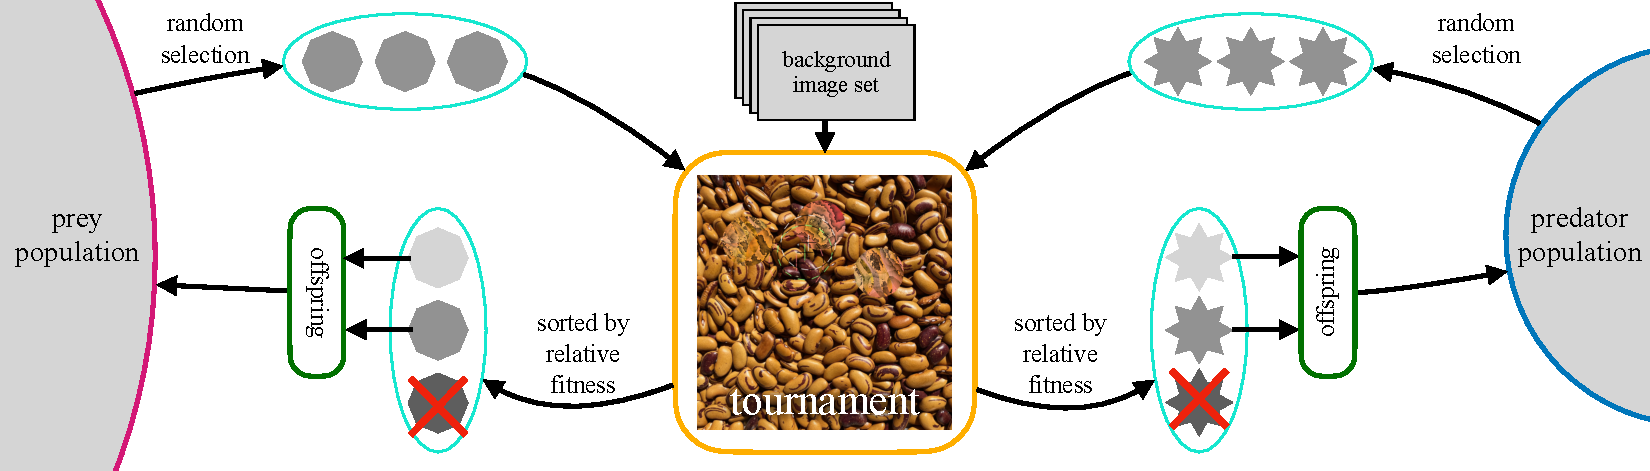
\includegraphics[width=\textwidth]{coc_overview.pdf}
    \caption{One step of the coevolutionary simulation of camouflage. \footnotesize (Three prey are selected at random from their population of 400. Similarly for three predators from their population of 40. A random background image is selected from the given set, and a random crop of 512² pixels is made. The three prey are rendered to random non-overlapping locations. This composite image is given to each predator which estimates a position (circled crosshairs in tournament image) predicting the most conspicuous prey's center. Predators are scored by “aim error”, distance from their estimate to the \jargon{ground truth} center of nearest prey. If the best predator's estimate is \textit{inside} a prey's disk, that prey is eaten and replaced by a new offspring of the other two prey. If all predators fail, all prey survive. If worst scoring predator misses all prey, it may die of starvation, replaced by a new offspring.)}
    \Description{Overview diagram of the coevolutionary simulation of camouflage evolution.}
    \label{fig:simulation_overview}
\end{figure*}

%%%%%%%%%%%%%%%%%%%%%%%%%%%%%%%%%%%%%%%%%%%%%%%%%%%%%%%%%%%%%%%%%%%%%%%%%%%

\begin{figure*}
    \igsix{20221030_1220_step_19.png}
    \hfill
    \igsix{20221030_1220_step_1045.png}
    \hfill
    \igsix{20221030_1220_step_2014.png}
    \hfill
    \igsix{20221030_1220_step_3059.png}
    \hfill
    \igsix{20221030_1220_step_6650.png}
    \hfill
    \igsix{20221030_1220_step_7467.png}
    \caption{Prey camouflage evolving over simulation time to become more effective in a given environment.}
    \Description{Sequence of images showing evolution of prey camouflage over simulated time.}
    \label{fig:time_sequence}
\end{figure*}

%%%%%%%%%%%%%%%%%%%%%%%%%%%%%%%%%%%%%%%%%%%%%%%%%%%%%%%%%%%%%%%%%%%%%%%%%%%

\section{Introduction}

Camouflage in nature seems to arise from competition between predator and prey. To survive, predators must find prey, and prey must avoid being found. This work simulates an abstract 2d model of that adversarial relationship. It looks at \jargon{crypsis} through evolving prey camouflage patterns (as procedural color textures) in competition with evolving predator vision (as a convolutional neural net) which learns to locate camouflaged prey. The environment for this 2D simulation is provided by a set of photographs, typically of natural scenes. This coevolutionary model has two evolving populations: one of prey and another of predators. See Figure \ref{fig:simulation_overview}.
\par
Prey evolve to be \jargon{cryptic} (hard to find) against the background. Evolving predators learn to hunt prey by locating their position. Mutual conflict between these populations produce both effective camouflage and skilled predators. The result is an open source \jargon{artificial life} model to help study camouflage in nature, and the perceptual phenomenon of camouflage more generally.
\par
Computational models of complex biological systems have several benefits. Constructing them, making them work as observed in nature, helps crystallize our thinking about natural phenomena. Computational models also allow experimentation \jargon{in silico} to help understand complex natural systems.
\par

%%%%%%%%%%%%%%%%%%%%%%%%%%%%%%%%%%%%%%%%%%%%%%%%%%%%%%%%%%%%%%%%%%%%%%%%%%%

\section{Approach}

This simulation follows the approach of \citet{reynolds_iec_2011}: a population of camouflaged prey evolve in response to negative selection from a predator seeking conspicuous prey. In that earlier interactive game-like simulation, the predator was a human “player.” 
\par
Here \cite{reynolds_coevolution_2023}, evolution of prey camouflage closely follows that earlier model. While the earlier human-in-the-loop predator is replaced here with a second population of predators, each based on a neural network. These CNN networks take an image (as in Figure \ref{fig:teaser}) as input and produce a \jargon{prediction}, an estimate, of where in the image the most conspicuous prey is located. Camouflage based on coevolution was first reported in \citet{harrington_coevolution_2014}.
\par
Prey evolution is simulated with \jargon{Genetic Programming}, an evolutionary algorithm that operates on a tree-structured “genome” which can represent expressions in a domain specific language. Here that language is the \href{https://github.com/cwreynolds/TexSyn}{TexSyn} library for procedural texture synthesis. Prey are removed from the population when “eaten” by a predator. They are replaced by \jargon{offspring} created with \jargon{crossover} between \jargon{parents} from the population. Similarly negative selection removes predators with low hunting success who die from “starvation”. During their lifetime, each predator learns its environment and the prey it has seen there. This is implemented by \jargon{fine tuning} its CNN. More model details and related work in \citet{reynolds_coevolution_2023}.
\par

%%%%%%%%%%%%%%%%%%%%%%%%%%%%%%%%%%%%%%%%%%%%%%%%%%%%%%%%%%%%%%%%%%%%%%%%%%%

\section{Simulations}

Simulations run for 12,000 steps, with 400 prey and 40 predators.  Each prey has a camouflage pattern, represented as a \jargon{tree} of TexSyn operators. Each predator has the same neural net architecture, with weights inherited from parents. Noisy weight copies and fine-tuning during their lifetimes lead to distinct optimization trajectories.
\par

%%%%%%%%%%%%%%%%%%%%%%%%%%%%%%%%%%%%%%%%%%%%%%%%%%%%%%%%%%%%%%%%%%%%%%%%%%%

\section{Conclusions}

Over simulated evolution time, patterns on prey \textit{seem} to become less conspicuous, as in Figure \ref{fig:time_sequence}. An objective measure is difficult due to the adversarial nature of the coevolutionary game. If predators stop finding prey, does that mean prey have gotten better, or that predators have gotten worse?
\par
Figure \ref{fig:sqm_plot} shows an objective metric based on a static predator model, pre-trained on a generic “find conspicuous disk” task. Predator fine-tuning during evolution is how they become better \jargon{specialists}. The \jargon{generalist} pre-trained predator is inherently weaker. Plots in Figure \ref{fig:sqm_plot} flatten over time. Is that because prey have stopped improving, or have they become too strong to be detected?
\par

Future work includes a better static quality metric, and to better understand why some background sets are “easy” and others “hard” (Fig. \ref{fig:sqm_plot}). This seems related to how \jargon{stationary} the background textures are, where different patches (say of a size comparable to prey) have the same statistical distribution of color and spatial frequency.
\par

%%%%%%%%%%%%%%%%%%%%%%%%%%%%%%%%%%%%%%%%%%%%%%%%%%%%%%%%%%%%%%%%%%%%%%%%%%%

\begin{figure}[b]
    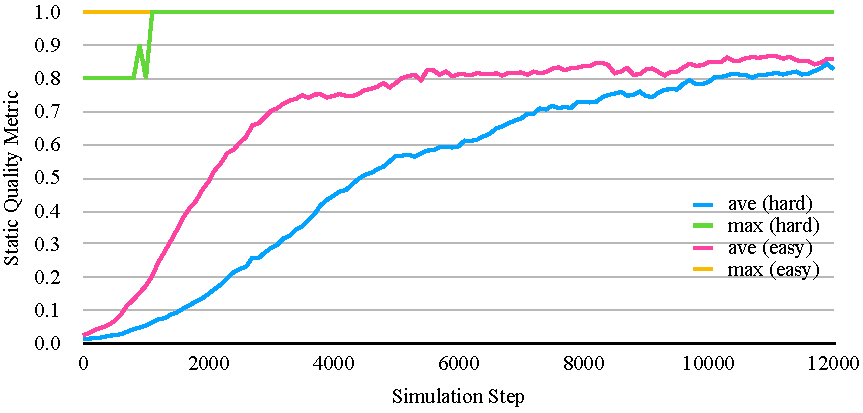
\includegraphics[width=\columnwidth]{SQM_plot_easy_vs_hard.pdf}
    \caption{Static quality metric versus simulation time.}
    % \Description{...}
    \label{fig:sqm_plot}
\end{figure}

%%%%%%%%%%%%%%%%%%%%%%%%%%%%%%%%%%%%%%%%%%%%%%%%%%%%%%%%%%%%%%%%%%%%%%%%%%%

%% Bibliography.
\bibliographystyle{ACM-Reference-Format}
\bibliography{coc.bib}

\end{document}